% IEEE LaTeX source derived from docs/janus-foundational-paper.md
% Note: Figure assets are referenced as placeholders (SVG inclusion may require conversion).

\documentclass[conference]{IEEEtran}

\usepackage[T1]{fontenc}
\usepackage[utf8]{inputenc}
\usepackage{lmodern}
\usepackage[final]{microtype}
\usepackage{xurl}
\usepackage{url}
\usepackage{tabularx}
\usepackage{tikz}
\usetikzlibrary{arrows.meta, positioning}
\usepackage{amsmath,amssymb}

\urlstyle{same}

\title{Janus: A Minimal Governance Kernel for\\
Deterministically Reconstructible\\
Human--AI Development Systems}

\author{\IEEEauthorblockN{Lic. Martín Nicolás Sánchez Morales}\\
\IEEEauthorblockA{Founder, Janus Governance Project\\
Argentina\\
\url{https://janusgovernance.org}}}

\begin{document}
\maketitle

\begin{abstract}
The rapid adoption of artificial-intelligence-assisted development tools has significantly transformed software engineering workflows. However, current technology governance frameworks primarily operate at organizational or regulatory levels---focusing on compliance, ethics, and risk management---while leaving the day-to-day governance of interactions between human developers and generative code systems largely undefined.

This paper introduces \textbf{Janus}, a minimal governance kernel for AI-assisted development environments. Janus defines a small set of foundational governance invariants that allow hybrid human--AI workflows to become \textbf{traceable, auditable, and deterministically reconstructible}.

The model is based on three foundational elements: append-only logs that preserve the institutional history of the system, an explicit dual evidence model ($E^{+}$ / $E^{-}$) capable of representing both recorded actions and verifiable omissions, and a formal boundary of human authority that maintains accountability for decisions requiring responsibility.

Unlike development methodologies such as Agile, DevOps, or ITIL, Janus does not redefine organizational processes. Instead, it introduces \textbf{minimal operational invariants} that stabilize the interaction between humans and generative systems without significantly increasing system complexity.

The result is a micro-structural intervention that can integrate with different technological stacks and reduce silent drift, ambiguity of authority, and loss of traceability in AI-assisted software development systems.
\end{abstract}

\begin{IEEEkeywords}
AI governance, human--AI systems, software governance, deterministic reconstruction, sociotechnical systems, development governance
\end{IEEEkeywords}

\section{INTRODUCTION}
Modern AI-based code generation tools---including conversational assistants integrated into development environments, automated copilots, and low-code automation platforms---have introduced a new production paradigm in software engineering.

This paradigm is characterized by:
\begin{itemize}
  \item external generation of technical artifacts
  \item accelerated iteration cycles
  \item reduced syntactic friction
  \item partial reliance on automated reasoning
\end{itemize}

However, this transformation introduces a structural problem that remains largely unexplored:

\textbf{How is the human--AI interaction governed at the micro-operational level of software development?}

Traditional methodologies regulate organizational processes, deployment pipelines, and workflow coordination, but they do not explicitly formalize the relationship between automated code generation and human validation.

This gap introduces structural risks such as:
\begin{itemize}
  \item diffuse authority
  \item undetected version drift
  \item validation based on plausibility
  \item absence of verifiable structural evidence
\end{itemize}

Janus emerges as a response to this governance gap.

\subsection{Contributions}
This paper makes three primary contributions:
\begin{enumerate}
  \item It proposes a \textbf{minimal governance kernel} for AI-assisted development environments.
  \item It introduces a \textbf{dual evidence model ($E^{+}$ / $E^{-}$)} capable of representing both recorded actions and structurally detectable omissions.
  \item It defines a \textbf{deterministic reconstruction model} that enables governance states to be rebuilt from governed events.
\end{enumerate}

These contributions aim to formalize micro-operational governance in hybrid human--AI systems without introducing additional organizational complexity.

\subsection{Research Hypothesis}
This work is grounded in the following hypothesis:

\textbf{In AI-assisted development systems, the absence of verifiable structural evidence generates operational drift, incoherence, and ambiguity of responsibility. Introducing a minimal set of governance invariants---based on append-only records, explicit evidence models ($E^{+}$ / $E^{-}$), and auditable human decisions---transforms plausibility-based workflows into deterministically reconstructible systems.}

In other words, the critical distinction is not merely between automation and human oversight, but between \textbf{believing that something occurred within a system and being able to demonstrate, through structural evidence, what actually occurred}.

Janus proposes a micro-structural intervention aimed at reducing this epistemic gap within hybrid human--AI systems. The underlying premise is that \textbf{small structural interventions can produce disproportionate improvements in the stability of complex systems}, particularly when human and machine actors share operational responsibility.

\section{THEORETICAL BACKGROUND}
\subsection{Sociotechnical Systems}
Sociotechnical systems theory states that the introduction of new technologies alters work organization and requires the redefinition of coordination and authority structures~\cite{trist1951}.

In AI-assisted development environments, the tool does not replace the developer; instead, it introduces an intermediate generative agent whose role and authority must be structurally defined. When generative systems participate directly in technical production, governance mechanisms must explicitly define how authority, validation, and responsibility are exercised across the human--AI boundary.

Within this context, the deterministic reconstruction model proposed by Janus also enables the preservation of \textbf{institutional memory} in hybrid socio-technical systems. Because governance events, evidence records, and human authority decisions are stored in append-only structures, the operational history of the system can be reconstructed over time without relying on informal recollection or fragmented documentation. In this sense, governance logs function not only as audit artifacts but as a durable record of institutional knowledge and decision history.

\subsection{Governance and Responsibility}
Governance involves the explicit definition of rules, responsibilities, and validation mechanisms within complex systems~\cite{kooi2003}. In software engineering literature, governance has also been examined at the architectural level, where architectural governance defines how system evolution and design decisions are supervised and validated across an organization~\cite{booch2006}.

In hybrid human--AI environments, the absence of clear operational rules may lead to reliance on informal trust or implicit authority.

Janus does not propose a general ethical framework but rather an operational model of technical governance.

\subsection{Infrastructure-Independent Architecture}
Clean architecture principles propose separating system rules from implementation technologies~\cite{martin2017}.

Janus adopts this approach by separating three components:
\begin{itemize}
  \item Normative core
  \item Executable runtime
  \item Interaction protocols
\end{itemize}

This architecture allows governance rules to remain independent of any specific technology.

\section{GOVERNANCE GAP IN AI-ASSISTED DEVELOPMENT}
In AI-assisted development workflows it is common to observe the following cycle:
\begin{enumerate}
  \item Requesting code from an AI system
  \item Inserting generated code into the development environment
  \item Iterating through trial-and-error
  \item Declaring success based on observable functionality
\end{enumerate}

This model may produce:
\begin{itemize}
  \item silent structural drift
  \item version fragmentation
  \item loss of traceability
  \item undocumented implicit validation
\end{itemize}

Artificial intelligence does not create these problems by itself; rather, it amplifies pre-existing structural weaknesses.

\section{JANUS: MICRO-OPERATIONAL GOVERNANCE}
Janus proposes a minimal governance layer based on the following principles:
\begin{itemize}
  \item Explicit authority
  \item Baseline freezing
  \item Validation gates
  \item Structured telemetry
  \item Structural identity validation
  \item Deterministic reconstruction
\end{itemize}

Janus does not impose an organizational methodology.

Instead, it defines \textbf{minimal structural invariants}.

\subsection{Governance Kernel}
Janus can be understood as a \textbf{minimal governance kernel} for hybrid human--AI systems.

This kernel defines only the foundational governance invariants necessary for maintaining traceability, auditability, and explicit responsibility.

\subsubsection{Append-Only Logs}
Three canonical logs store the system’s institutional history:
\begin{itemize}
  \item MANAGEMENT\_LOG
  \item SCHEMA\_LOG
  \item AUDIT\_LOG
\end{itemize}

\subsubsection{Evidence Model}
The system distinguishes between two types of evidence:
\begin{itemize}
  \item \textbf{$E^{+}$} --- explicitly recorded evidence
  \item \textbf{$E^{-}$} --- evidence derived from the verifiable absence of an expected record
\end{itemize}

\subsubsection{Governance Evaluation}
Evaluation processes interpret evidence within a defined scope to determine whether governance events must be generated.

\subsubsection{Governance Events}
Janus defines two canonical events:
\begin{itemize}
  \item OMISSION\_DETECTED
  \item HUMAN\_DECISION
\end{itemize}

\subsubsection{Authority Boundary}
Governance events may only be written through an authorized mechanism known as the \textbf{Audit Writer}.

\subsubsection{Deterministic Reconstruction}
Governance state can be reconstructed from:
\begin{itemize}
  \item historical logs
  \item schema context
  \item evidence references
\end{itemize}

\section{EVIDENCE MODEL ($E^{+}$ / $E^{-}$)}
A central contribution of Janus is the introduction of a dual evidence model.

\subsection{Positive Evidence ($E^{+}$)}
Records actions that effectively occurred.

\subsection{Negative Evidence ($E^{-}$)}
Records detectable omissions: expected actions that did not occur within a defined structure.

This model allows representing not only events that occurred but also \textbf{structurally relevant absences}.

\begin{figure}[ht]
\centering
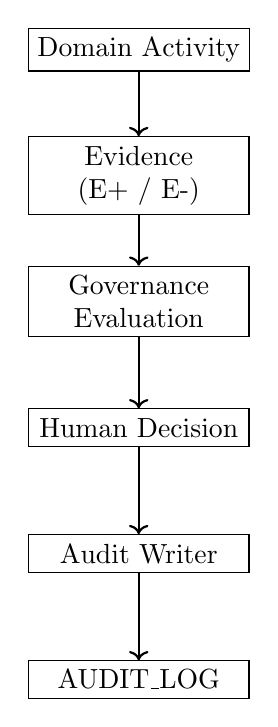
\begin{tikzpicture}[
node distance=1.6cm,
every node/.style={draw, rectangle, align=center, minimum width=2.8cm},
arrow/.style={->, thick}
]

\node (domain) {Domain Activity};
\node (evidence) [below of=domain] {Evidence\\(E+ / E-)};
\node (evaluation) [below of=evidence] {Governance\\Evaluation};
\node (human) [below of=evaluation] {Human Decision};
\node (audit) [below of=human] {Audit Writer};
\node (log) [below of=audit] {AUDIT\_LOG};

\draw[arrow] (domain) -- (evidence);
\draw[arrow] (evidence) -- (evaluation);
\draw[arrow] (evaluation) -- (human);
\draw[arrow] (human) -- (audit);
\draw[arrow] (audit) -- (log);

\end{tikzpicture}
\caption{Janus Governance Kernel Pipeline. Domain activity generates evidence (E+ / E−), which is interpreted by governance evaluation flows. When accountability is required, explicit human authority produces a HUMAN\_DECISION event. Governance outcomes are recorded through the authorized Audit Writer into AUDIT\_LOG, enabling deterministic reconstruction of governance state.}
\label{fig:janus_pipeline}
\end{figure}

\subsection{Conceptual Formalization}
\begin{equation}
\mathrm{GovernanceState} = f(\mathrm{Event},\, \mathrm{Evidence},\, \mathrm{HumanDecision})
\end{equation}

Where:
\begin{itemize}
  \item \textbf{Event} represents domain events occurring in the system
  \item \textbf{Evidence} represents evidence generated under the $E^{+}$ / $E^{-}$ model
  \item \textbf{HumanDecision} represents explicit human authority decisions
\end{itemize}

A second relation captures deterministic reconstruction:
\begin{equation}
\begin{split}
\mathrm{GovernanceState}_{t} = g(\mathrm{MANAGEMENT\_LOG}_{\le t},\\
\mathrm{SCHEMA\_LOG}_{\le t},\, \mathrm{AUDIT\_LOG}_{\le t})
\end{split}
\end{equation}

This equation expresses that the governance state at time \textbf{$t$} can be deterministically reconstructed from the canonical logs of the system.

Evidence itself can be defined as:
\begin{equation}
\mathrm{Evidence} = E^{+} \cup E^{-}
\end{equation}

Together, these relations show that governance in Janus does not rely on implicit states but on reconstructible functions derived from observable records.
\begin{equation}
\mathrm{SystemState} = h(\mathrm{GovernanceState})
\end{equation}

This relation expresses that, when governance events fully describe authorized system activity, the operational state of the system becomes derivable from the governance state itself. In other words, deterministic reconstruction assumes that governance events capture the set of authorized operational transitions within the system.

\begin{figure}[ht]
\centering
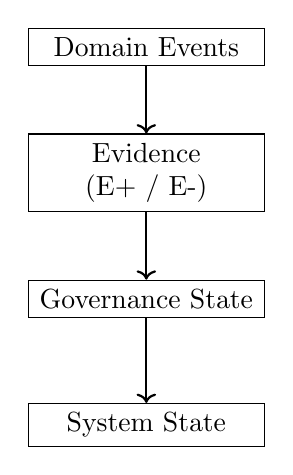
\begin{tikzpicture}[
node distance=1.6cm,
every node/.style={draw, rectangle, align=center, minimum width=3cm},
arrow/.style={->, thick}
]

\node (events) {Domain Events};
\node (evidence) [below of=events] {Evidence\\(E+ / E-)};
\node (gov) [below of=evidence] {Governance State};
\node (system) [below of=gov] {System State};

\draw[arrow] (events) -- (evidence);
\draw[arrow] (evidence) -- (gov);
\draw[arrow] (gov) -- (system);

\end{tikzpicture}
\caption{Socio-Technical System Reconstruction Model implied by the Janus governance kernel. Domain events generate evidence (E+ / E−), which is evaluated through governance processes. Human authority decisions and audit-controlled logging produce a governance state from which the operational system state becomes derivable.}
\label{fig:janus_reconstruction}
\end{figure}

\section{INITIAL EMPIRICAL VALIDATION}
A relevant methodological characteristic of the project is that the development of Janus itself---including the conceptual core, code repositories, documentation environment, and experimental runtimes---was conducted under the same governance protocols proposed by the system.

In this sense, the project functioned as an initial case of \textbf{structural self-governance (dogfooding)}, where traceability rules, event recording, and human decisions were applied during the system’s own construction.

This approach allowed the internal coherence of the model to be evaluated in real AI-assisted development conditions.

In methodological terms, \textbf{Janus was developed under its own governance constraints}, reinforcing the alignment between the proposed model and its experimental implementation.

The model was tested through:
\begin{itemize}
  \item definition of a runtime-independent core
  \item implementation in an Apps Script runtime
  \item implementation in a Node runtime
  \item structured telemetry testing focused on verifying deterministic reconstruction of governance state from append-only logs and detecting structural inconsistencies through the $E^{+}$ / $E^{-}$ evidence model
\end{itemize}

Observed results include:
\begin{itemize}
  \item structural stability
  \item contract coherence
  \item structural detection of inconsistencies
  \item controlled reproducibility
\end{itemize}

\section{DISCUSSION}
Although Janus is presented primarily as a \textbf{minimal governance kernel}, its design allows higher layers to evolve toward a broader \textbf{governance framework for AI-assisted development environments}.

This paper does not claim the existence of such a framework but instead describes the \textbf{minimal foundational governance invariants} that could support future extensions. In alignment with this objective, the Janus core is intended to be distributed as an \textbf{open-source governance kernel}, allowing independent researchers and engineering teams to reproduce experiments, audit the governance model, and implement alternative runtimes while preserving the canonical governance invariants defined in this work.

In this sense, Janus may be understood as a conceptual infrastructure upon which policies, tools, and governance runtimes could be constructed while preserving the simplicity of the proposed kernel.

Janus does not compete with organizational governance frameworks nor attempt to replace agile methodologies or architectural governance models described in the literature~\cite{booch2006}.

Instead, it operates at a different level: the \textbf{micro-operational layer of human--AI interaction}. At this level, deterministic reconstruction also implies that governance records function as a persistent institutional memory of the system, preserving the traceable history of decisions, evidence, and authority.

\subsection{Conceptual Comparison}
A central aspect of Janus is how it differs from existing models.

Most frameworks used in software engineering operate at different levels of the problem addressed in this work.

Methodologies such as \textbf{Agile, DevOps, and ITIL} regulate organizational processes and delivery cycles. Systems such as \textbf{Git} provide historical integrity of source code. Contemporary \textbf{AI governance frameworks} often focus on ethical, regulatory, or institutional dimensions, such as the NIST AI Risk Management Framework~\cite{nist2023}.

Janus instead operates at the \textbf{micro-operational level of human--AI interaction during technical production}.

Its distinctive characteristics include:
\begin{enumerate}
  \item \textbf{Evidence-based governance} through the $E^{+}$ / $E^{-}$ model
  \item \textbf{Deterministic reconstruction of governance state} via append-only canonical logs
  \item \textbf{Explicit separation between technical generation and human authority} through auditable decision events
\end{enumerate}

\begin{table}[ht]
\caption{Conceptual comparison}
\label{tab:comparison}
\centering
\setlength{\tabcolsep}{3pt}
\renewcommand{\arraystretch}{1.05}
\begin{tabularx}{\columnwidth}{l X X X}
\hline
Concept & Versioning & Organizational Governance & Janus \\
\hline
System History & commits & process documentation & append-only logs \\
Integrity & hashes & institutional audit & controlled audit writing \\
Validation & pull requests & hierarchical approval & HUMAN\_\allowbreak{}DECISION \\
Evidence & commit history & reports & E+ / E- \\
Reconstruction & checkout & documentary reconstruction & deterministic reconstruction \\
Operational Level & code organization & human governance & human–AI interaction \\
\hline
\end{tabularx}
\end{table}

\section{LIMITATIONS}
Janus:
\begin{itemize}
  \item does not guarantee system security
  \item does not replace regulatory compliance
  \item does not eliminate human error
  \item does not substitute organizational ethical frameworks
\end{itemize}

Its scope is deliberately limited.

\section{CONCLUSION}
The integration of artificial intelligence into software development introduces new ambiguities regarding authority, responsibility, and validation.

While existing governance frameworks operate primarily at institutional levels, the everyday interaction between human developers and generative systems remains largely under-formalized.

Janus proposes a micro-governance layer designed to address this operational gap. Rather than introducing complex infrastructures, Janus defines a small set of foundational governance invariants capable of stabilizing hybrid human--AI systems.

The central hypothesis is that \textbf{small structural interventions can produce disproportionate improvements in the stability of complex systems}.

Similar to how distributed version control, code review practices, and continuous integration reshaped software engineering culture, a minimal governance layer may help reduce silent drift, ambiguity of responsibility, and traceability loss in AI-assisted development.

Janus therefore aims not to replace existing governance frameworks but to complement them by addressing the micro-operational layer where human and machine collaboration actually occurs.

If governance events fully describe authorized system activity, the operational state of the system becomes derivable from the governance state. In this sense, governance records are not merely audit artifacts but may function as a reconstructible structural description of system operation.

This interpretation highlights a broader implication of the model: governance infrastructure can also operate as a durable mechanism for preserving institutional memory in socio-technical systems. By recording governance events, evidence structures, and explicit human decisions, the system preserves a reconstructible history of institutional knowledge and operational responsibility.

\begin{thebibliography}{00}
\bibitem{trist1951} E.~L. Trist and K.~W. Bamforth, ``Some Social and Psychological Consequences of the Longwall Method,'' \emph{Human Relations}, 1951.
\bibitem{kooi2003} J. Kooiman, \emph{Governing as Governance}. Sage Publications, 2003.
\bibitem{martin2017} R.~C. Martin, \emph{Clean Architecture: A Craftsman's Guide to Software Structure and Design}. Prentice Hall, 2017.
\bibitem{nist2023} National Institute of Standards and Technology, ``AI Risk Management Framework (AI RMF 1.0),'' NIST, 2023.
\bibitem{booch2006} G. Booch, ``Architectural Governance in Software Systems,'' \emph{IEEE Software}, 2006.
\end{thebibliography}

\end{document}
